\section{Siamese Multi-Object Tracking and Attention}
\label{sec:SiamMOTandAttention}

\subsection{Motivation}

\subsection{Deformable Convolutional Neural Networks}
\label{ssec:DeformableCNNS}

\Glspl{dcnn}~\cite{dai2017dcnn} are gaining popularity and are being applied to numerous sophisticated computer vision tasks, e.g., object segmentation (dense predictions) and object detection (semi-dense predictions). Since object tracking revolves around the same requirements in terms of pixel-wise precision, we contemplated using this advancement as well.

Although \glspl{cnn} (\sectionstr{}~\ref{ssec:ConvolutionalNeuralNetworks} on page~\pageref{ssec:ConvolutionalNeuralNetworks}) are an excellent tool for a plethora of deep learning tasks involving image processing, they are still limited in their capabilities to model a broad range geometric transformation. To address this, practictioners apply a broad range of data augmentation techniques (e.g., rotation, translation, scaling, and shearing) to provide the necessary samples of some particular transformation during the training. However, such approach is limited to tailor-made transformations that may not cover the entire set of possibilities the model may face in practice. Also, there is a large body of literature on designing transformation invariant features~\cite{lowe1999sift, rublee2011orb}. We also encountered scale and rotation equivariant Siamese trackers that inherently handled the two transformations.

The first work to learn spatial transformation from the training data in a deep learning fashion is known under the name \glspl{stn}~\cite{jaderberg2016stn} by Jaderberg~\etal{}. It warps the feature map via a global parametric transformation such as affine transformation

% ------------------------------------------------------------------------------
\begin{figure}[t]
    \centerline{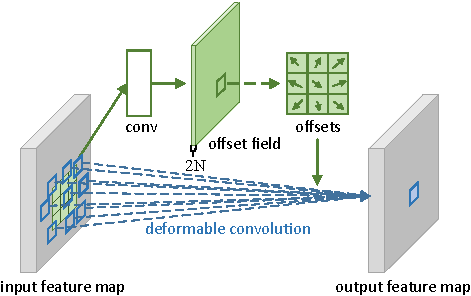
\includegraphics[width=0.6\linewidth]{figures/methodology/deformable_convolution.pdf}}
    \caption[\Gls{dcnn}]{ \externalsrc{\cite{dai2017dcnn}}}
    \label{fig:FCOSCenterness}
\end{figure}
% ------------------------------------------------------------------------------
